\hypertarget{interfaceorg_1_1newdawn_1_1slick_1_1util_1_1pathfinding_1_1_mover}{}\section{org.\+newdawn.\+slick.\+util.\+pathfinding.\+Mover Interface Reference}
\label{interfaceorg_1_1newdawn_1_1slick_1_1util_1_1pathfinding_1_1_mover}\index{org.\+newdawn.\+slick.\+util.\+pathfinding.\+Mover@{org.\+newdawn.\+slick.\+util.\+pathfinding.\+Mover}}
Inheritance diagram for org.\+newdawn.\+slick.\+util.\+pathfinding.\+Mover\+:\begin{figure}[H]
\begin{center}
\leavevmode
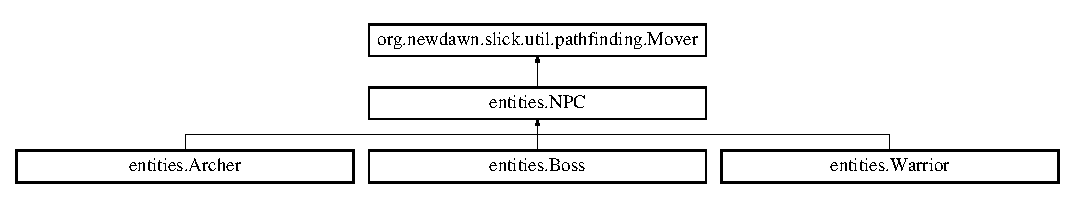
\includegraphics[height=2.222222cm]{interfaceorg_1_1newdawn_1_1slick_1_1util_1_1pathfinding_1_1_mover}
\end{center}
\end{figure}


\subsection{Detailed Description}
A tagging interface for an object representing the entity in the game that is going to moving along the path. This allows us to pass around entity/state information to determine whether a particular tile is blocked, or how much cost to apply on a particular tile.

For instance, a \mbox{\hyperlink{interfaceorg_1_1newdawn_1_1slick_1_1util_1_1pathfinding_1_1_mover}{Mover}} might represent a tank or plane on a game map. Passing round this entity allows us to determine whether rough ground on a map should effect the unit\textquotesingle{}s cost for moving through the tile.

\begin{DoxyAuthor}{Author}
Kevin Glass 
\end{DoxyAuthor}
